\documentclass[12pt, a4paper]{article}
\usepackage[utf8]{inputenc}
%\usepackage{Times}
\usepackage{authblk}
\usepackage{setspace}
\usepackage{apacite}
\usepackage{caption}
\usepackage{graphicx}
\usepackage[margin=1in]{geometry}
\pagestyle{myheadings}
\title{}
\author{}
\date{}
\doublespacing

\usepackage{color}

\definecolor{orange}{rgb}{1,0.7,0.7}
\newcommand{\NS}[1] {{\textcolor{green}{#1}}}
\newcommand{\AT}[1] {{\textcolor{cyan}{#1}}}
\newcommand{\TM}[1] {{\textcolor{orange}{#1}}}

\title{Zero attraction: A precisely zero attraction effect with naturalistic stimuli that meets Huber, Payne, and Puto's (2014) criteria}

\author{Anna Trendl\\Department of Psychology, University of Warwick \and Neil Stewart and Timothy L. Mullett\\Warwick Business School, University of Warwick}

\date{\today}

\begin{document}

\begin{titlepage}
\maketitle

\newpage

\begin{abstract}
In the attraction effect, adding a third option to a choice set of two options can reverse the preference for the original options and even increase the choice share of one of the original options. The attraction effect bears significant importance for decision-making research, as it is a violation of the axioms of regularity and independence from irrelevant alternatives, which are core properties of any model in which the utility of each option is stable across choice sets. Consequently, the attraction effect has driven the development of a set of influential models of multiattribute choice in the past 20 years. Recently, \citeA{Frederick2014} claimed that the attraction effect is limited to options presented as collections of numerical attributes, and does not hold for choices between naturalistic options like snacks or movies---a claim which would severely undermine the importance of the effect for the development of models of choice. \citeA{Huber2014} criticised \citeauthor{Frederick2014}'s experiments, laying down a set of strict criteria that should be met by any experiment wishing to test for the attraction effect in choices involving naturalistic choice options. We present the first experiment that meets these criteria. We find a precisely zero attraction effect.
\end{abstract}
\end{titlepage}

\NS{Neil has comments like this}

\AT{Anna has comments like this}

\TM{Tim has comments like this}


\section{To Do}

0. \NS{Style guide}: "alternative" not "option"? Choose one and stick to it.

1. Add in text explaining why the attraction effect is important: The attraction effect is important because it rules out the simple scalable family of models, where the value of each alternative is independent of the choice set in which it appears. For the introduction of the decoy to reverse preferences between the target and the comparison is a violation of independence of irrelevant alternatives and often of regularity, where the introduction of a new alternative to a choice set cannot increase the choice share on any existing alternative. Because of its theoretical importance, it has played a significant role in the development of multialternative models of choice, with a significant number quite different theoretical accounts being developed in the past 20 years {cite them all, from MDbS}. For this reason, it would be of considerable importance if the attraction effect is confined only to numerical stimuli presented in an attribute by alternative format. Arguably, while choices in the real world involve stimuli are often presented in a rich naturalistic form \cite{Bhatia2018b}, most experiments which have been used to develop theory use the numerical attribute x alternative format. There are substantial differences in decision making with these naturalistic stimuli. For example, Bhatia and Stewart (2018) show that the heuristic chice strategies that are so well supported by  the numerical attribute x alternative experiments are substantially outperformed by a simple weighted additive regression when naturalistic stimuli are used. \AT{Done}

2. Highlight that although the stimulus set construction is weird, it is all validated by the ratings then choice data from the experimental session after the preregistration. Something upfront like "While the details of our stimulus construction are necessarily somewhat arbitrary, this does not undermine the quality of the experiment. We were able to check, using only the responses from the experimental session after stimulus construction and preregistration that our triplets meet every one of the the Huber et al. requirements."

3. Add the list of stimuli, the preregistration, the data, and the R script to an OSF page so we are sharing everything up front. Don't make public yet. 
\section{Introduction}

%\AT{\textbf{Dessert version}}

Imagine that you are having a nice meal in a restaurant, and you are looking at the two dessert options available on the menu: cheesecake and pecan pie. You are torn between the creamy texture of the cheesecake and the rich, nutty flavour of the pecan pie. You resolve to have the cheesecake. As the waiter approaches to take your order, he informs you that a third dessert option, apple pie---which you find quite bland---is also available today. But now you have changed your mind, and decide to order the pecan pie. \citeA{Tsetsos2010} give just this paradoxical example: the availability of the apple pie, which you do not want, makes you switch from cheesecake to pecan pie.

This is an example of the attraction effect (also known as asymmetric dominance effect). The presence of the apple pie (decoy) in the choice set makes you more likely to choose the pecan pie (target) over the cheesecake (competitor). In essence, it states that when the decision maker is indifferent between the target and the competitor (pecan pie and cheesecake in the example), the addition of an inferior decoy option that resembles the target (apple pie is similar to pecan pie, but is less liked by the decision maker) increases the likelihood that the target will be chosen.


The attraction effect is important, because it poses a challenge to all choice models that rely on the assumption that preferences can be represented on a cardinal utility scale. This assumption is called simple scalability, and is one of the consequences of Luce's choice axiom \cite{Luce1959}. Crucially, the attraction effect represents a violation of independence of irrelevant alternatives, which requires that the preference ranking of two options should not be affected by adding new options to the choice set. In addition, the attraction effect violates the axiom of regularity, which states that an option's choice probability cannot increase when the choice set is extended (\citeNP{Luce1977a}; \citeNP{Tversky1972a}). Therefore, the existence of the attraction effect means that utility of a choice option cannot be represented by a single internal magnitude that is invariant to the other options in the choice set. 

Owing to its theoretical importance, the attraction effect has played a substantial role in the development of multialternative models of choice, with a significant number of quite different theoretical accounts having been proposed over the past 20 years (e.g., multialternative decision field theory, \citeNP{Roe2001a}; leaky competing accumulators, \citeNP{Usher2004b}; multialternative attentional drift-diffusion model,   \citeNP{Krajbich2010a}; range-normalization model, \citeNP{Soltani2012}; associative accumulation model, \citeNP{Bhatia2013b}; multiattribute linear ballistic accumulator, \citeNP{Trueblood2014a}; multialternative decision by sampling, \citeNP{Noguchi2018a}). 

The first multiattribute choice experiments (e.g., \citeNP{Huber1982}; \citeNP{Simonson1992}) often used stimuli presented as a set of numerical attributes (e.g., cars presented as numerical values for gas mileage and ride quality). However, recent experiments in multiattribute choice introduced what can perhaps be considered as more ecologically valid stimuli (e.g., movies presented as thumbnails and titles on Netflix or photographs of popular snacks). Results from these experiments indicate that there might be significant differences in the processing of numerical and naturalistic stimuli. For example, \citeA{Bhatia2018b} find that, with naturalistic stimuli, the weighted additive model on a high-dimensional semantic representation generalises to new choices better than the simpler heuristic models, which perform so well on stimuli presented as sets of numerical attributes. 

Recently, the existence of the attraction effect in choices that involve naturalistic options has become a contentious issue.
\citeA{Frederick2014} presented a thorough investigation of the boundary conditions of the attraction effect based on 38 experiments. These stimuli types included choice options with numerically represented attributes as well as complex, real-world stimuli (e.g., fruits, bottled water, apartments, etc.), and in some of these experiments participants could even sample the choice options (e.g. squash, mints, popcorn). The overall conclusion of this study was that while the presence of the decoy seemed to affect decisions with numerical stimuli, it was absent in experiments with more complex, naturalistic stimuli. In light of these results, \citeauthor{Frederick2014} posited that the psychological processes underlying decisions that involve options with numeric attributes are fundamentally different from those employed in decisions where the stimuli has a naturalistic representation. This conclusion was also supported by \citeA{Yang2014}, who reported difficulties replicating the attraction effect when the stimuli were pictorial, as opposed to when attributes were presented numerically.

These two studies sparked considerable interest amongst decision making researchers, and led to the re-examination of the boundary conditions of the attraction effect. \citeA{Huber2014} discussed five critical conditions that can inhibit the attraction effect, and argued that many of these are present in the experiments reported by \citeauthor{Frederick2014} and \citeauthor{Yang2014}. The five critical conditions are to avoid: (1) strong prior preferences over the target and competitor, (2) an inability to identify the dominance relationship  between the target and the decoy, (3) heterogeneity in prior preferences over the target and competitor, (4) an undesirable decoy and (5) a decoy that is too desirable. \citeA{Simonson2014a} further stressed the importance of the detection of the dominance relationship in observing the attraction effect, and also pointed out several other smaller, specific methodological shortcomings of the studies by \citeauthor{Frederick2014} and \citeauthor{Yang2014}.

Due to the theoretical significance of the attraction effect, it is important to know if the attraction effect is confined to choice settings with numerical stimuli presented in an attribute by alternative format. Arguably, while most consumer choices in the real world involve stimuli that are often presented in a rich naturalistic form \cite{Bhatia2018b}, development of formal models of choice have been almost exclusively reliant on results from experiments where the options have a numerical attribute by alternative format. In this article, we describe a test of the attraction effect with complex, naturalistic choice options, using an experimental methodology that addresses all of the critical conditions discussed by \citeA{Huber2014}. Using a movie choice task, we find no evidence for the attraction effect. We discuss the implications of our findings for understanding the boundary conditions of the attraction effect.

\section{Testing the attraction effect with real-world stimuli}
%not sure what's the naming convention with just 1 experiment

The goal of this experiment was to test the attraction effect with naturalistic stimuli. We chose to use the most popular movies on IMDb as stimuli. Since movies are an integral part of Western culture, we can reasonably expect that most our participants will be sufficiently interested in the choice options. Furthermore, choosing between movies is a realistic, everyday task, and this way we can mimic real-world decision making. In addition, the movie space is rich enough so that we can create a wide range of unique choice triplets to test the attraction effect.

When the stimuli has numerical attributes, it is straightforward to construct choice triplets with a target, competitor and decoy. However, with naturalistic stimuli, this task is significantly more complicated. \citeauthor{Frederick2014} have also used movie stimuli in two of their experiments: they chose pairs of movies that are part of the same sequel or are starring the same actor (but have distinctly different genres) to create target-decoy pairs. In the movie sequel version, they assumed that the second part of the sequel is the decoy, and the first part is the target, whereas in the movie actor experiment it is unclear how they decided which movie of the same actor should be the target and the decoy. We believe that this experimental approach has a significant flaw.

Specifically, there is no guarantee that the participants perceived the triplets as they were intended by the authors: whether \textit{Grease 2} will be perceived as inferior to \textit{Grease} (or the other way around) is completely up to the decision maker's preferences, which they did not control for. Individual heterogeneity in preferences can severely alter the perception of real-world choice triplets, thus, it is imperative to take it into account in the choice triplet selection.

Our novel experimental design takes individual preferences into account, and thus ensures that decision makers are both indifferent between the target and competitor and are able to clearly identify the inferiority of the decoy. In addition, to increase the statistical power of our test, we used a within-subjects design as well as both A, B, A' and B, A, B' triplet pairs (where X' is the dominated option), as suggested by \citeA{Huber2014}. We created "quadruplets" (each made up of two attraction effect choice triplets), using two distinctly different target-decoy pairs. Figure \ref{fig:quadruplets} shows an example of two choice triplets created from one such quadruplet.


 \begin{figure}
\centering
\captionsetup{justification=centering}
		 \caption{Two choice triplets used in the experiment.}
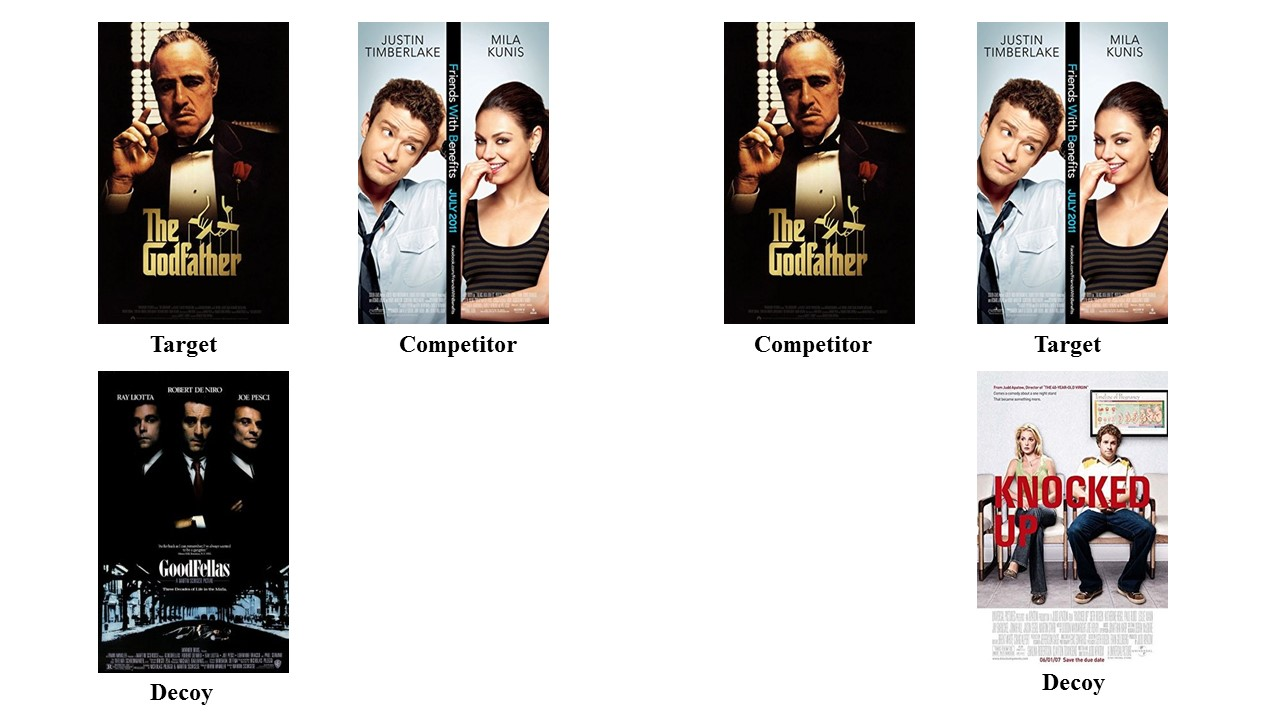
\includegraphics[width=1\textwidth]{figure1.jpg}
\label{fig:quadruplets}
\end{figure}

\subsection{Method}

\subsubsection{Pre-Registration}
The study design, exclusion criteria and all the analyses were planned and registered before we collected any choice data. The pre-registration can be accessed at \NS{Insert link to OSF page}.

\subsubsection{Candidate choice set selection}

Our movie triplets are listed in \NS{Table X in the Appendix}. The details of the construction of these triplets are somewhat arbitrary---a different recipe could have been use. However,the key issue is that our triplets pass \citeauthor{Huber2014}'s \citeyear{Huber2014} criteria, as we detail below.

We first retrieved the most popular 40 movies from each of 10 distinct genre categories (romance, drama, sci-fi, thriller, comedy, horror, animation, fantasy, crime, action) from IMDb, so that we had 400 movies overall. We chose a wide range of genres to obtain a sufficiently rich stimuli space. We omitted an sequels.

Owing to the multidimensional nature of the stimuli, one of the main difficulties in creating attraction effect choice triplets from real-world objects is establishing a criterion for matching up similar objects. We used genre and sub-genre information from allmovie.com to create target-decoy pairs with overlapping genres that are likely to be perceived as similar and to create target-competitor pairs with non-overlapping genres that are likely to be perceived as different.

We conjectured that it will be harder to find movie pairs that will be perceived as similar because any given movies is similar to a only a few movies and dissimilar to all of the others. For this reason, we started the quadruplet creation with selecting potential target-decoy pairs.

The genre information on allmovie.com is very rich: compared to the 18 genre categories on IMDb, there are 156 genre and sub-genre categories, capturing many important aspects of the movies. Using this rich genre information, we created a movie by movie ($400 \times 400$) matrix, where each cell was the number of overlapping genre categories between the two movies. We select as target-decoy pairs all of the pairs where, for a given target movie, the number of overlapping genres with a candidate decoy was equal to the maximum overlap seen for that target across all candidate decoy movies, creating 2,271 target-decoy candidates.
We also added 806 movie pairs obtained from the mutually closest 10\% of movies based on a latent semantic analysis\footnote{The latent semantic analysis assesses the similarity of two items based on the text associated with them. For this analysis, we used the summary text about the movies as well as plot keywords, actor and director names, all retrieved from IMDb.} that were not already in our list of target-decoy candidates. The rationale behind using semantic proximity as an additional criterion was to capture movie pairs that are very close to each other in terms of the story themes, but are not the closest on the genre dimension. Overall, we had 3,011 unique target-decoy candidate pairs at this point.

We then reduced the size of this list by selecting the most similar movie pairs. This was done manually by two researchers, who gave a similarity rating between 1--7 for each movie pair (1-least similar, 7-most similar). We only kept the movie pairs that had a similarity rating above 1, weeding out the movie pairs that were obviously not similar, resulting in 1,242 target-decoy candidates. We then divided the 1,242 pairs into six groups of 207 pairs and ran a pilot study where we asked 60 participants to rate the similarity of a randomly chosen group of movie pairs, obtaining 10 independent similarity ratings for each of the 1,242 target-decoy candidates. Participants rated the similarity of each movie pair on the 1--7 scale which also included a ``don't know'' option. Figure \ref{fig:exp2_pilot}  shows the distribution of the average similarity ratings for each movie pair.

\begin{figure}[htb!]
\centering
\captionsetup{justification=centering}
		\caption{The distribution of the average similarity rating for each target-decoy candidate pair (N = 1242). The dotted line is the cut-off value for accepting a movie pair as similar.}
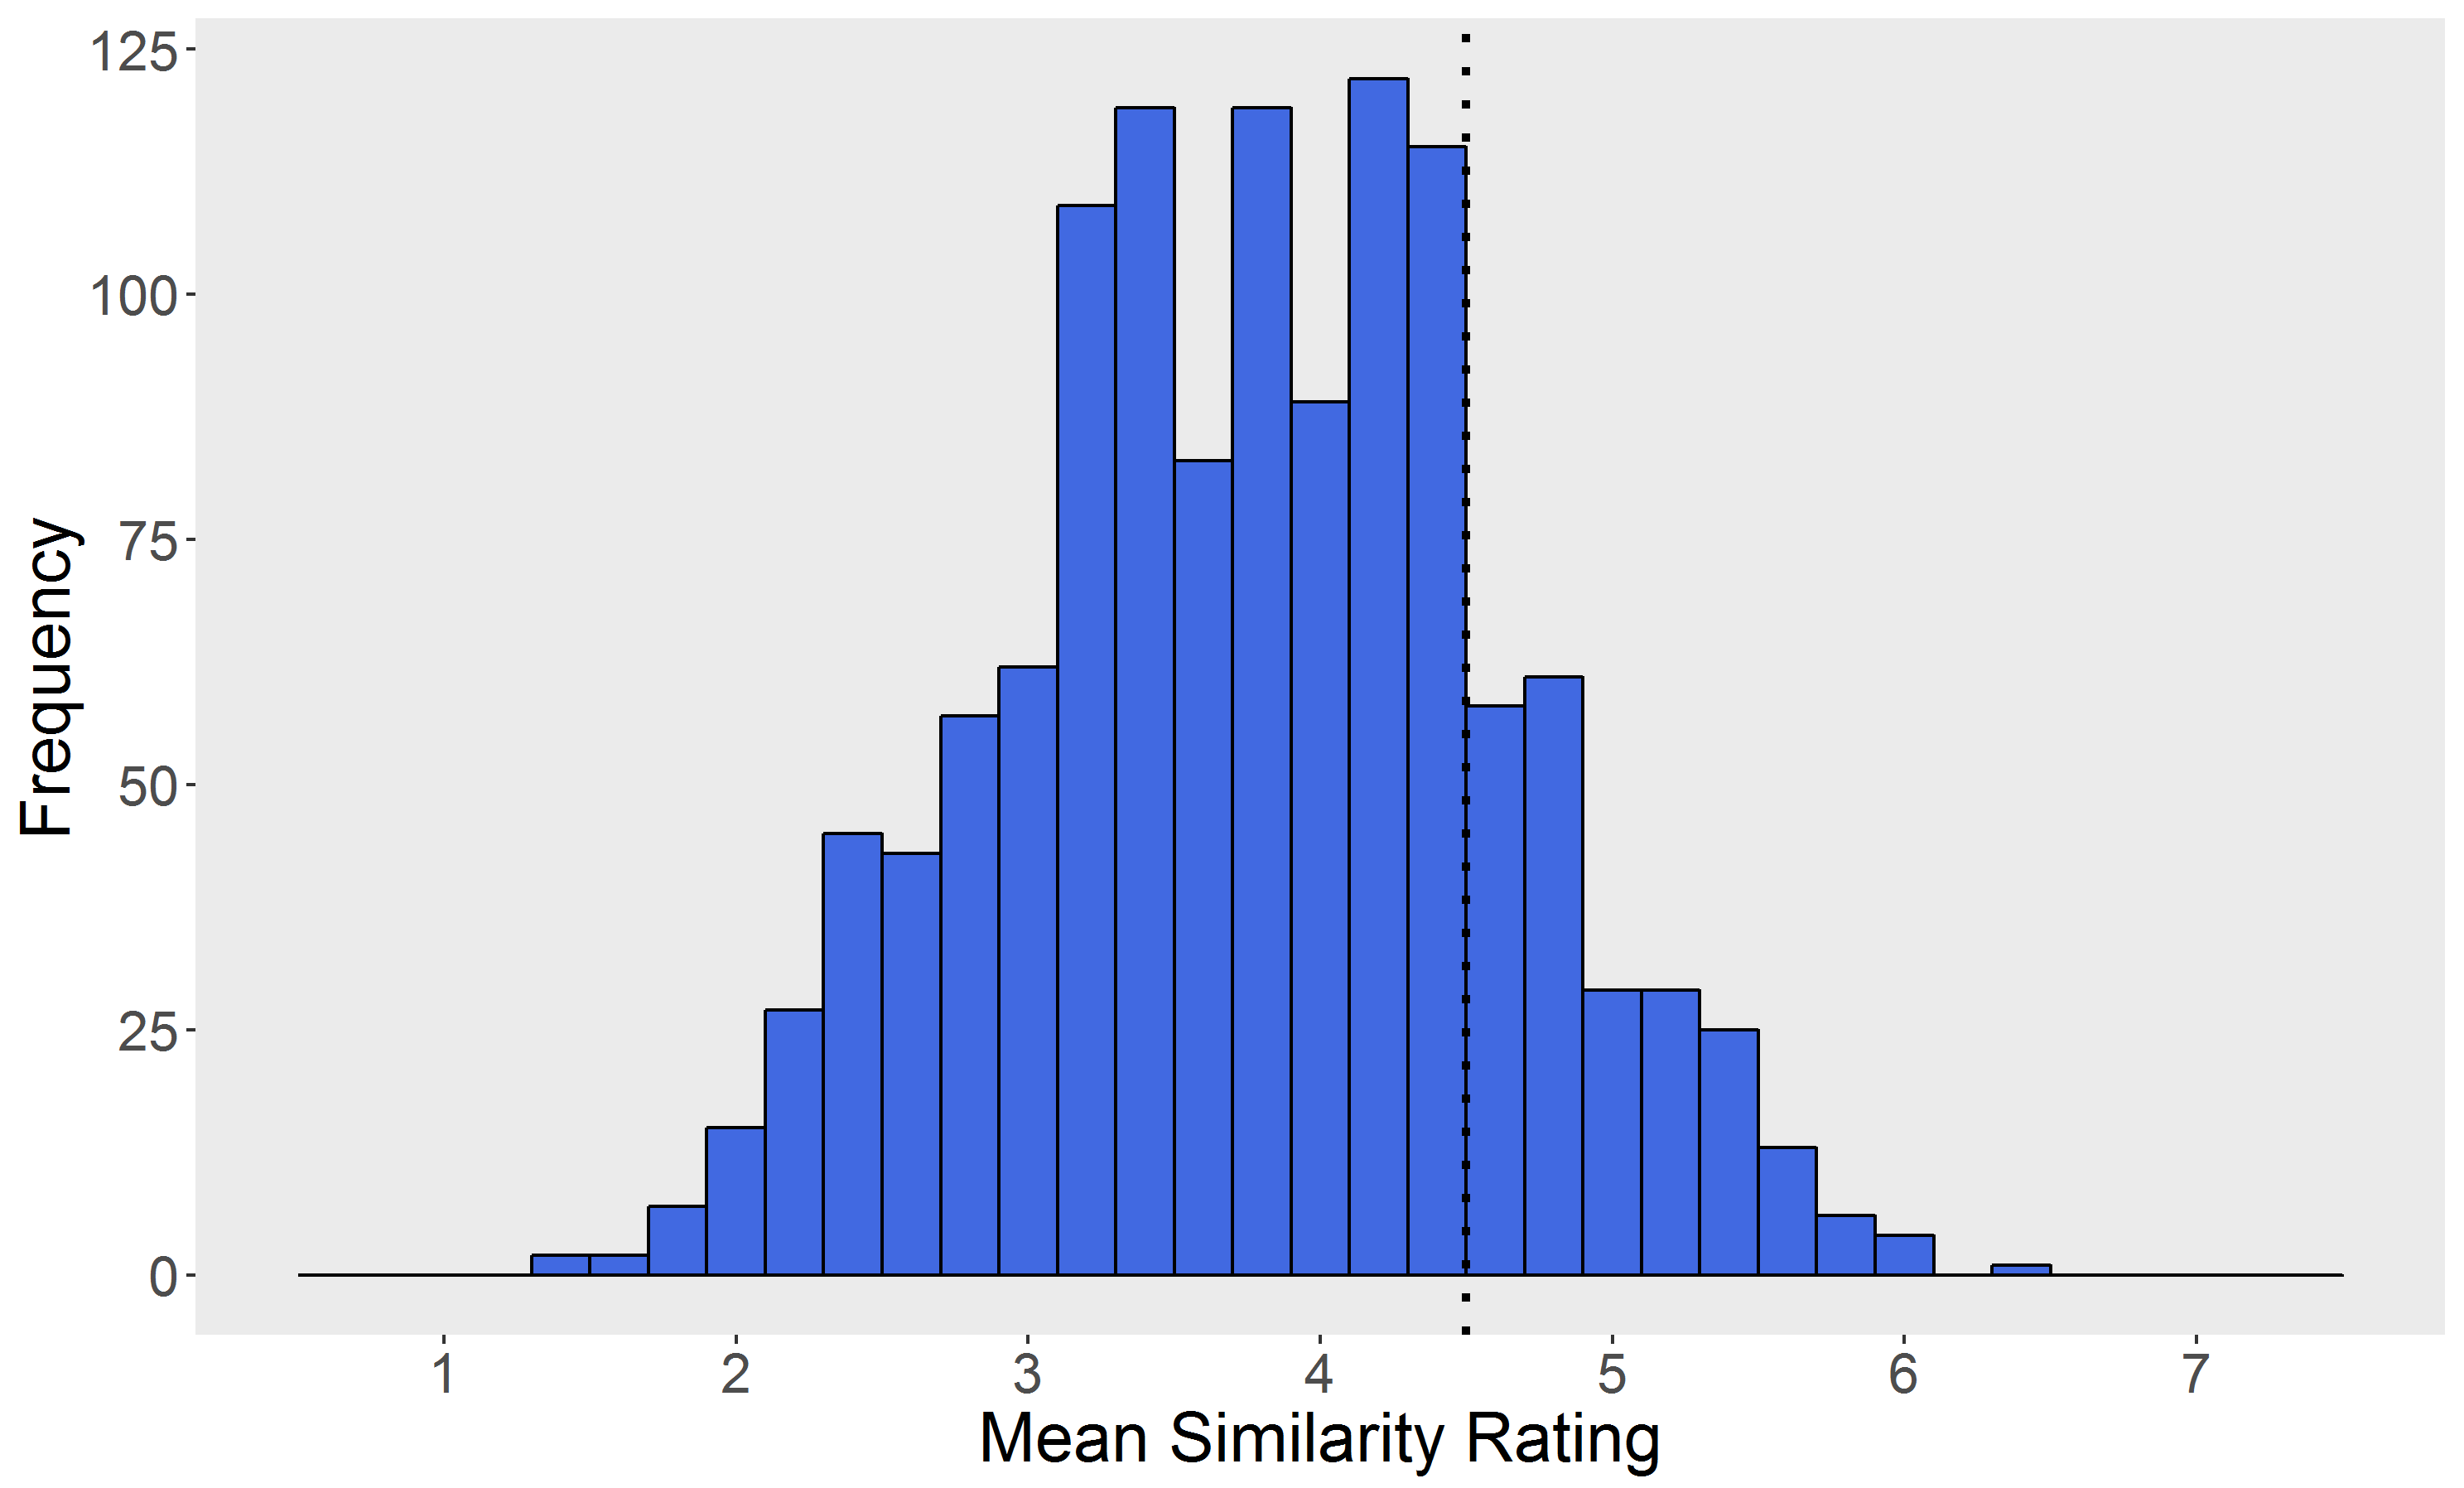
\includegraphics[width=0.9\textwidth]{exp2_pilot.png}
\label{fig:exp2_pilot}
\end{figure}

We decided to only use movie pairs with ratings that are equal to or higher than 4.5, which corresponds to the upper 20\% of the similarity rating distribution (253 movie pairs). We intended this procedure will ensure that our target-decoy pairs will be perceived as similar by most people.

The next step in creating the quadruplets was to create target-competitor pairs. Since each quadruplet consists of two target-decoy pairs (Movies A and B and Movies C and D in Figure \ref{fig:quadruplets}), we decided to pair up the 253 target-decoy pairs to create the quadruplets. To do this, we first created a target-decoy pair by target-decoy pair matrix (253x253), where each cell was the number of overlapping genre categories between the two movie pairs. For example, considering the comparison between target-decoy candidate 1 (consisting of Movie A and Movie B) and target-decoy candidate 2 (consisting of Movie C and Movie D), we summed the number of genre overlaps between movies A-C, A-D, B-C and B-D. We then selected the unique target-decoy pairs that had no genre overlap with each other. This resulted in 20,022 quadruplets, each of which is a combination of four movies, created from 231 unique movies. The quadruplets used for each participant are based upon their own ratings of the 231 movies, as we describe below.

\subsubsection{Experimental Procedure}

The experiment consisted of three stages: rating stage, choice stage, similarity rating stage. In the rating stage, we asked for participants' subjective evaluations over the 231 movies (``How do you personally rate this movie?'') on a scale from 1 (worst) to 7 (best). We also asked whether the participant had seen the movie before. The 231 movies were presented in a random order for each participant. The rating stage took about 15--20 minutes.

Before the choice stage, we created a bespoke set of movie triplets for each participant using their ratings from the rating stage. First, based on the ratings from the first stage, we identified the subset of quadruplets where: (a) the target and competitor were both rated 4, both rated 5, both rated 6, or both rated 7, and (b) the two decoy movies were rated at least 3 points lower than the two decoy candidates. Note that we did not require the two decoys in the quadruplet to have the same rating as it would have severely limited the number of quadruplets we could use (e.g., we allowed for quadruplets with ratings 7,7 for the two targets and 4,1 for the two decoys), but we controlled for this difference in our analysis.

We then selected the subset of quadruplets where all of the movies had been seen or none of the movies had been seen, to make sure that choice behaviour will not be governed by differences in familiarity with the movies. The result was a bespoke subset of quadruplets for each participant where the target/competitor movies had the same rating and the decoy movies were rated worse. However, we did not want the same movie to appear twice as a target/competitor for one participant, and for this reason we used a sequential elimination technique: we first chose the quadruplet with the highest combined target-decoy similarity rating, then eliminated all quadruplets with the same target/competitor movies. We repeated these steps until we had a set a of quadruplets with unique target/competitor movies.

We only invited those participants back for whom we could create at least three unique quadruplets (corresponding to at least six attraction effect choice triplets). In the choice task, people were presented with the selected movie triplets in a random order and were asked to choose the one they liked the most (see Figure \ref{fig:exp1_screenshot}).

\begin{figure}[htb!]
\centering
\captionsetup{justification=centering}
\caption{Choice stage.}
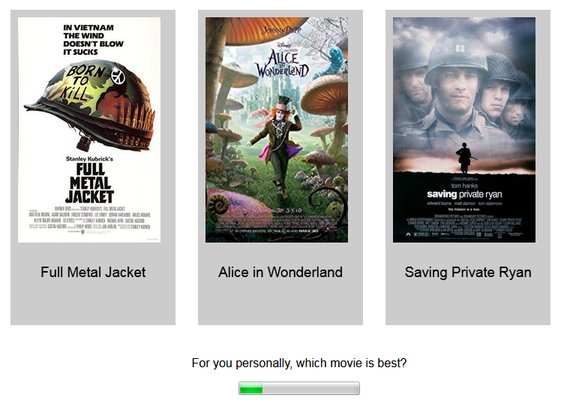
\includegraphics[width=0.8\textwidth]{rsz_exp1_choicestage.png}
\label{fig:exp1_screenshot}
\end{figure}

In the final, similarity stage, we asked participants to rate the similarity of all target-decoy and target-competitor pairs on a scale from 1 (least similar) to 7 (most similar), where a "don't know" option was also included. Information collected in this similarity rating stage was important to check that out choice participants each perceived the similarity between the movie pairs as we intended.

We collected data in batches of 50 until we had choice data for at least a 100 participants (after all the exclusion criteria had been applied, see section \ref{exclusion_ref}). At most a few days passed between the rating and choice stage. We recruited 297 participants from Prolific Academic who were paid £8 per hour. Out of the 297 participants that completed the rating stage, we could create quadruplets for 179 of these participants. Out of the 179 participants who were invited back, 152 took part in the choice stage of the experiment.

\subsubsection{Exclusion criteria} \label{exclusion_ref}

To conduct a rigorous test of the attraction effect, it is crucial that people take the task seriously and reveal their true preferences. Given that individually rating 231 movies can seem somewhat mundane, we specified a set of exclusion criteria to filter those people out who did not take the rating task sufficiently seriously. These were the following. We excluded people who fell into the fastest 5\% of the reaction time distribution, the lowest 5\% of the entropy distribution and the upper and lower 5\% of the autocorrelation distribution. Entropy refers to the diversity of the ratings, while autocorrelation takes into account the temporal pattern and measures the extent to which a response depends on previous responses. Thus, this procedure filtered out response patterns where people (a) spent an unusually short time completing the task or (b) did not use the whole of the ratings scale or (c) often gave the same ratings for consecutive movies or (d) were giving ratings randomly.

These exclusion criteria were validated in a pilot study, where we collected ratings for a set of books and included repeat trials. The participants filtered out by these three criteria are the ones who give the least consistent ratings to repeated stimuli (correlation $r < 0.8$).

We applied these exclusion criteria to our sample of 152 people, excluding 17 people, leaving a sample of 135 participants.


\subsubsection{Results}

The average number of choice trials per participant was 16 (the lowest being 6 and the highest 54), and 84\% of participants were presented with at least 8 choice trials.

The decoy was only chosen in 4.3\% of the trials. In addition, 72\% of the participants have never chosen it, and only 2\% of people have chosen it in more than 25\% of the trials. This indicates that people were able to identify the dominated decoy in the choice stage.

To test for the presence of the attraction effect, we first excluded all trials where the decoy was chosen and then conducted a one-sample t-test to test the hypothesis that the mean of the proportion of trials where the target was chosen is above 0.5 (indicating an increased likelihood of choosing the target item). We found no evidence for the attraction effect (M = 0.5, SD = 0.07), t(134) = -0.44, p = .669. Figure \ref{fig:exp2_res} shows the distribution of the proportions of trials where the target was chosen, which shows that participants were almost perfectly indifferent between the target and the competitor, M = 0.5, 95\% CI [0.49, 0.51].



\begin{figure}[htb!]
\centering
\captionsetup{justification=centering}
\caption{Proportion of trials where the decoy was chosen. Each dot is a participant and the red dot and error bars show the bootstrapped mean and 95\% CIs.}
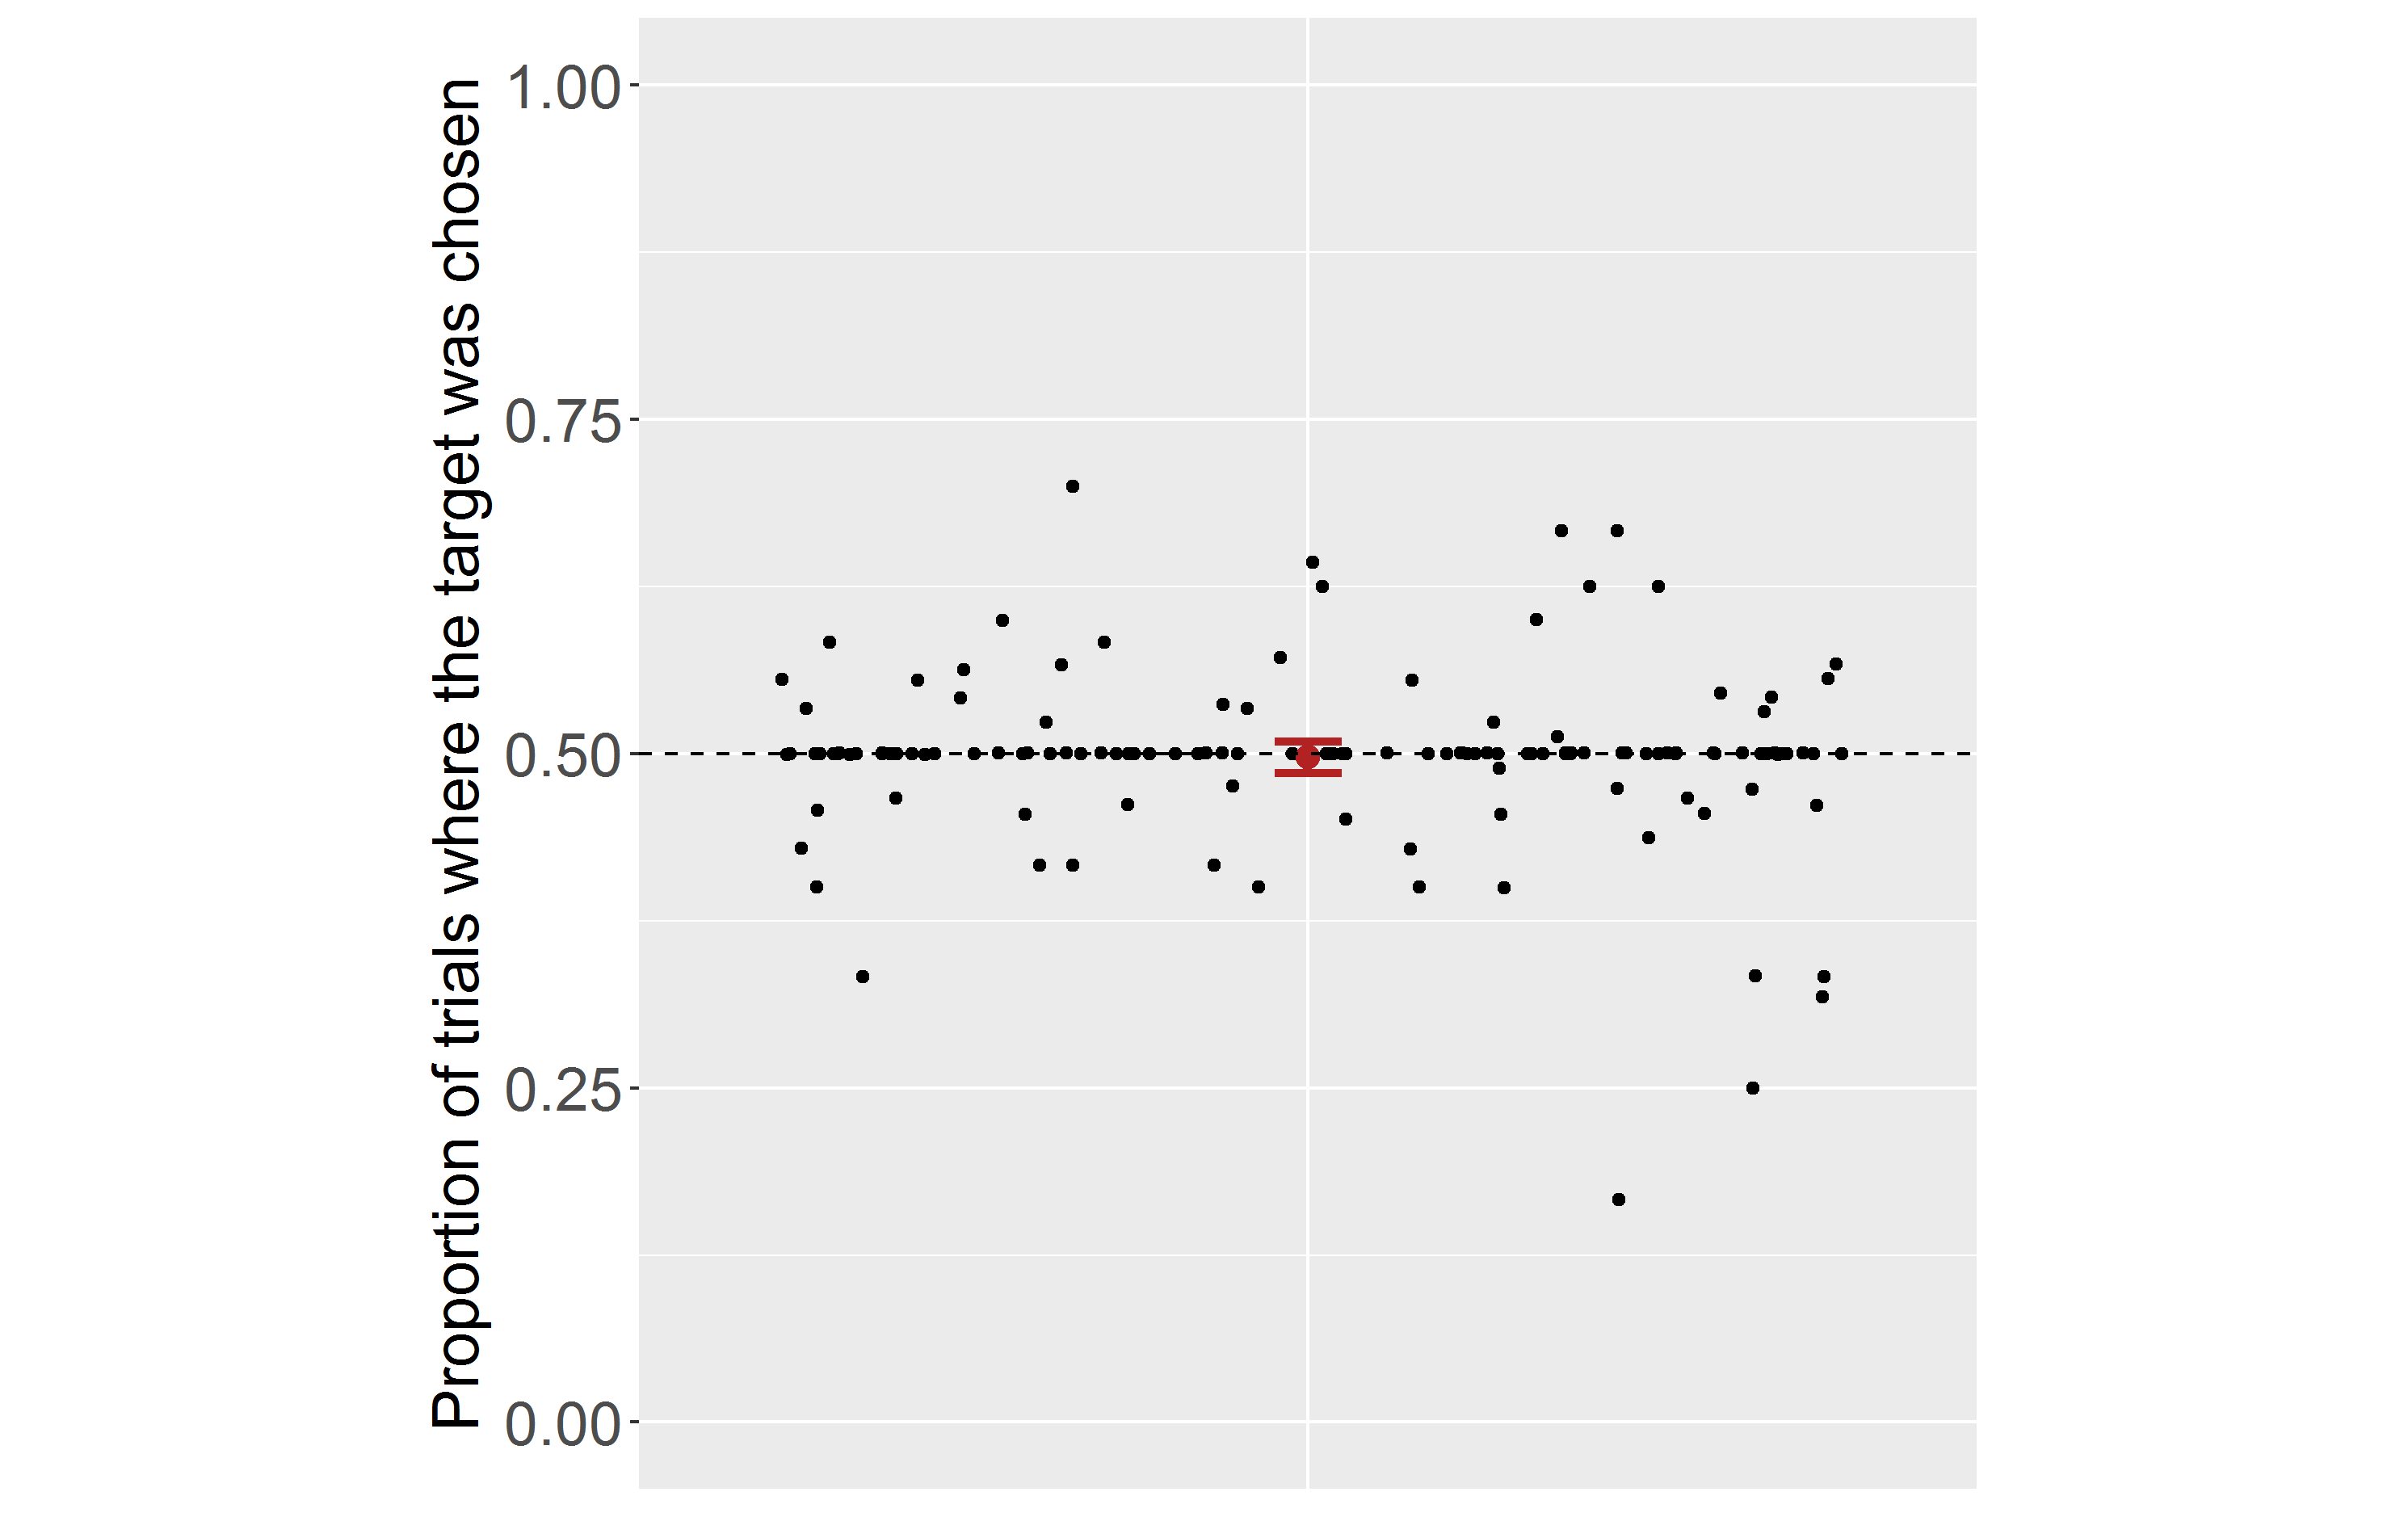
\includegraphics[width=0.8\textwidth]{exp2_res.png}
\label{fig:exp2_res}
\end{figure}

While we crated the choice triplets very carefully to ensure that they actually represent an attraction effect choice situation where the target-decoy pairs are perceived as similar and the target-competitor pairs perceived as different, individual heterogeneity and malleable preferences can still affect the results. Therefore, we find it instructive to plot the target-decoy and target-competitor similarity rating distributions. Figure \ref{fig:exp2_similarityratings} shows these distributions, and we can see that the overwhelming majority of target-competitor pairs were perceived as not similar, while the majority of target-decoy pairs were perceived as similar, as we hoped.

\begin{figure}[htb!]
\centering
\captionsetup{justification=centering}
\caption{Distribution target-competitor and target-decoy similarity ratings.}
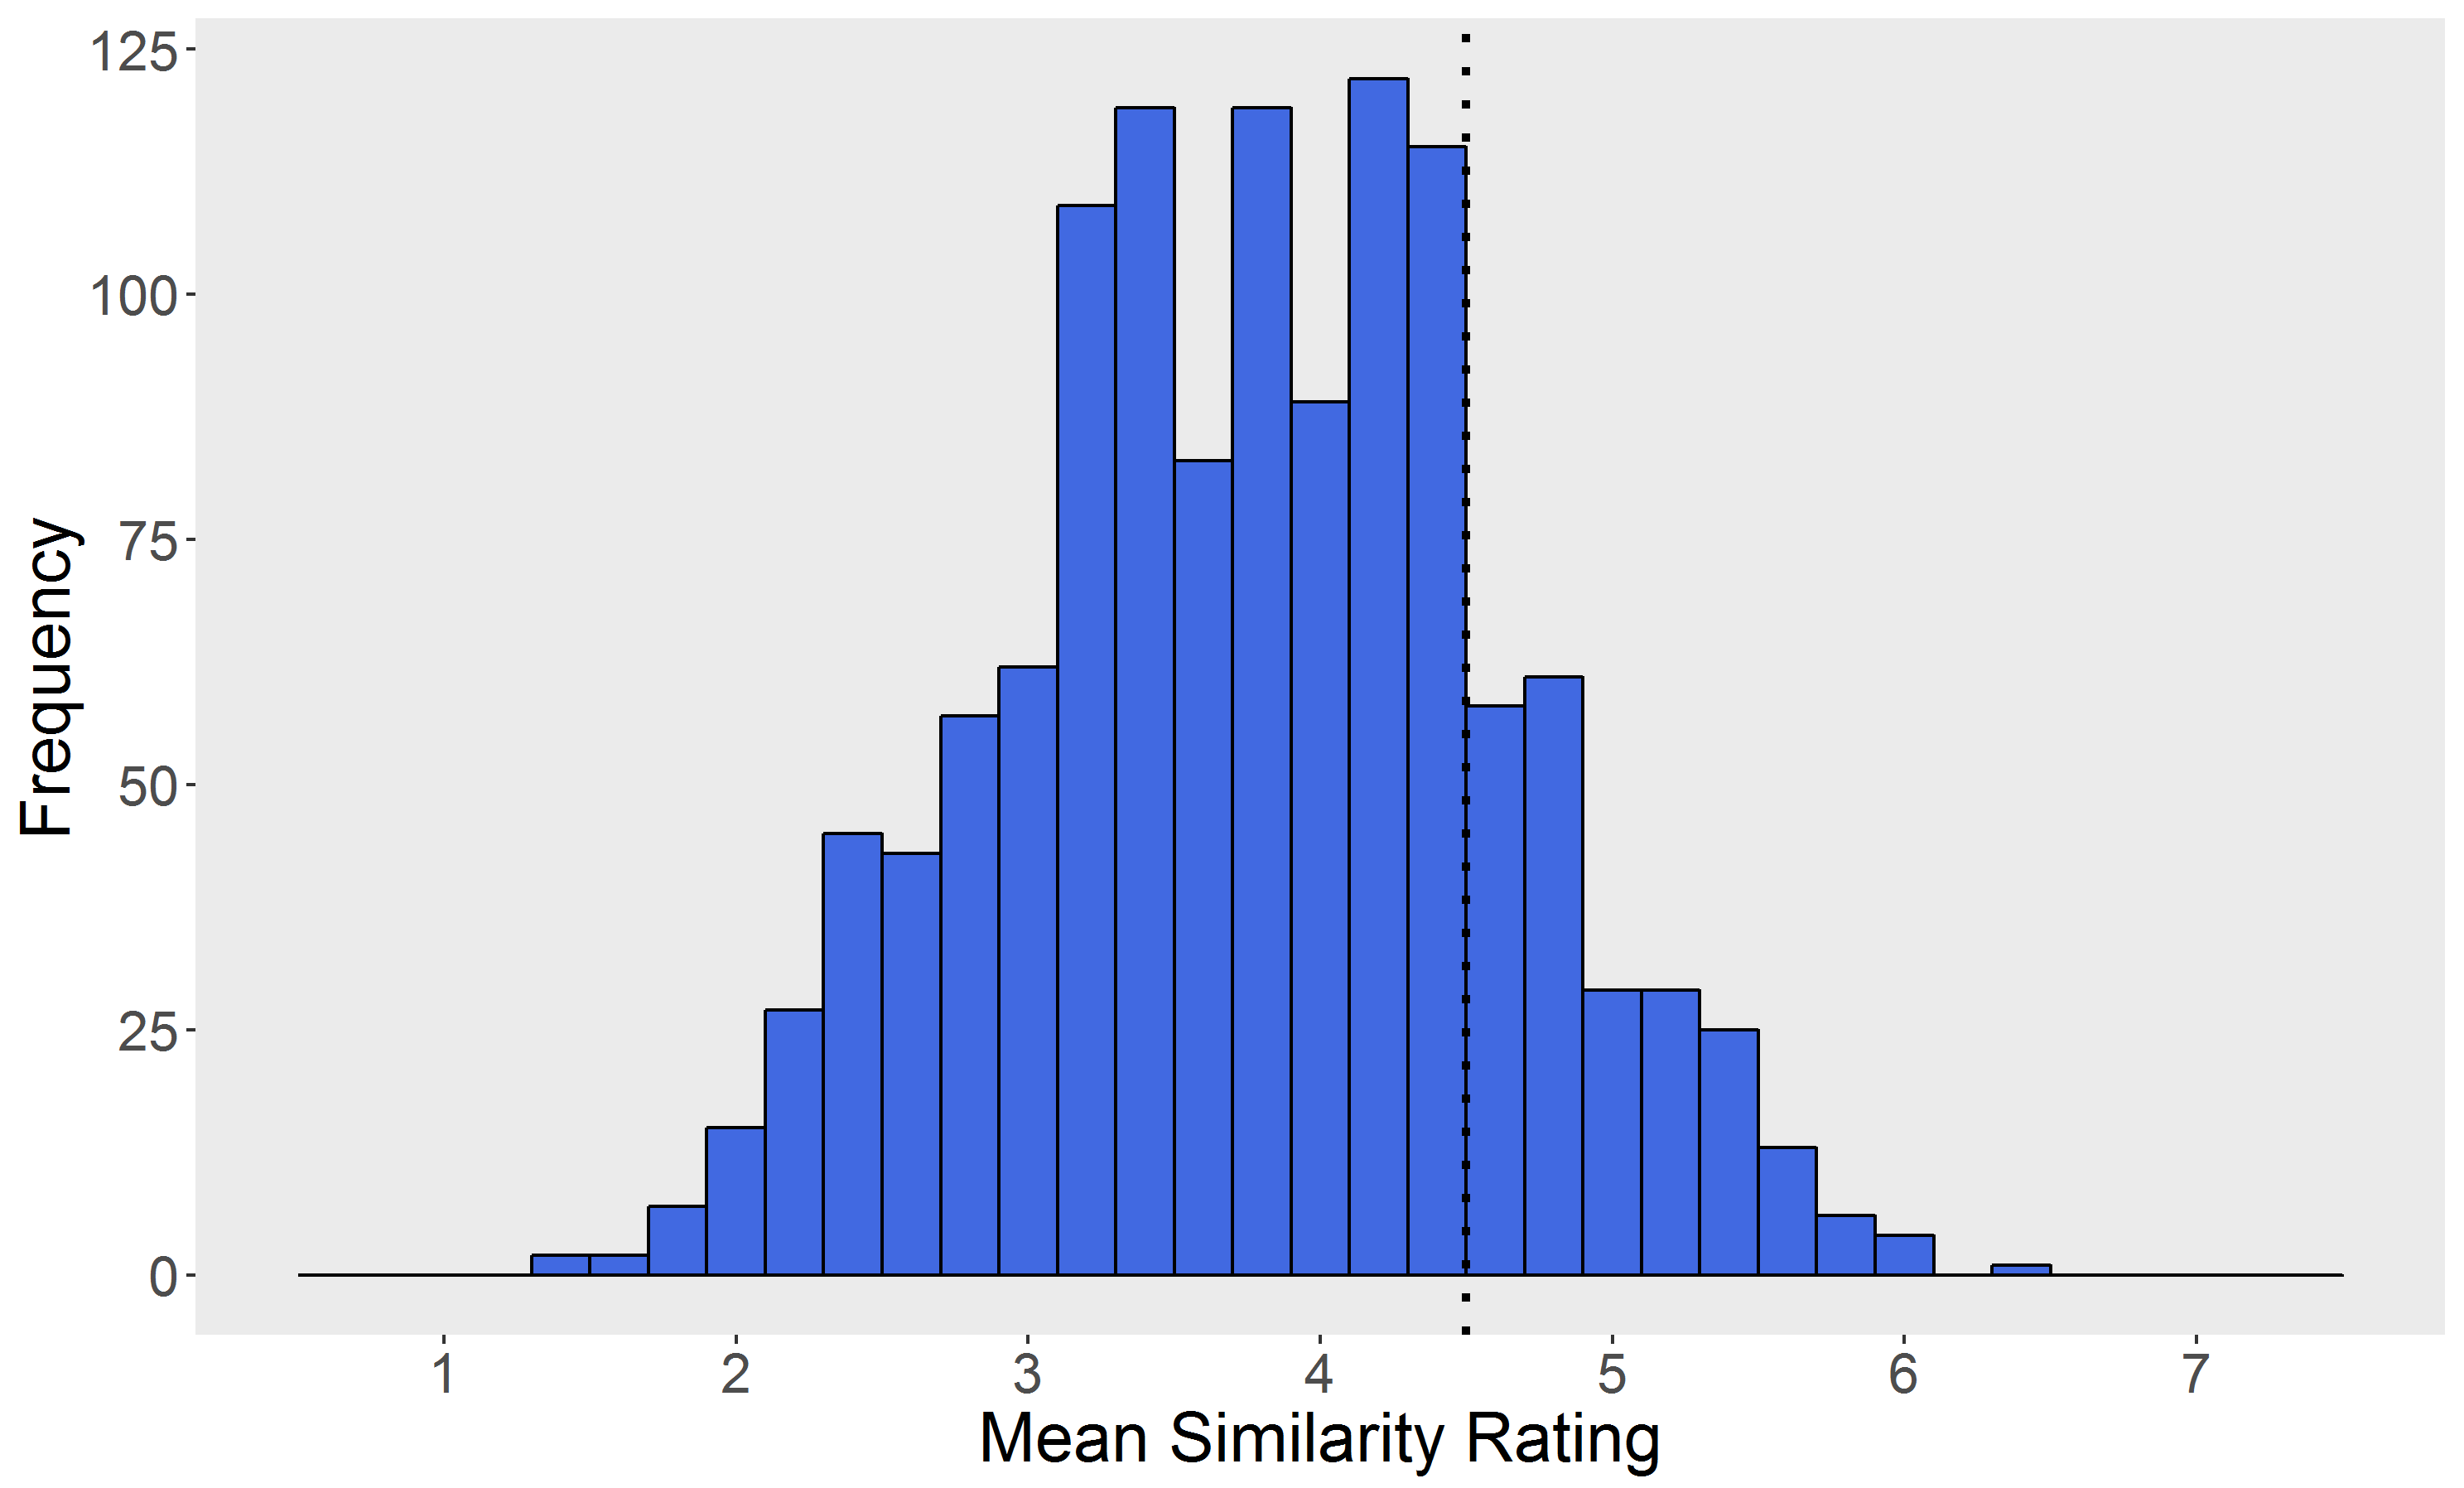
\includegraphics[width=0.8\textwidth]{exp2_similarityratings.png}
\label{fig:exp2_similarityratings}
\end{figure}

As specified in our pre-registered analysis plan, we also ran a mixed effects logistic regression with subject-specific intercepts to investigate how subjects' target-decoy and target-competitor similarity ratings and familiarity with the movies affects the likelihood of choosing the target. Table \ref{latentattr_exp2reg} shows the results from this regression, where contrary to our expectations, none of the explanatory variables seem to modulate the strength of the attraction effect.

\begin{table}[!htbp] \centering
\captionsetup{justification=centering}
  \caption{Odds-ratios and 95\% CIs from a mixed-effects logistic model with subject-specific intercepts. (T - Target, C - Competitor, D - Decoy)}
  \label{latentattr_exp2reg}
\resizebox{9cm}{!}{\begin{tabular}{@{\extracolsep{5pt}}lc}
\\[-1.8ex]\hline
\hline \\[-1.8ex]
 & \multicolumn{1}{c}{\textit{Dependent variable:}} \\
\cline{2-2}
\\[-1.8ex] & Target chosen \\
\hline \\[-1.8ex]
 Seen all & 1.122 (0.731, 1.729) \\
  TC similarity rating & 0.967 (0.872, 1.073) \\
  TD similarity rating & 0.926 (0.835, 1.027) \\
  TD rating difference & 0.935 (0.837, 1.044) \\
  Intercept & 1.062 (0.598, 1.882) \\
 \hline \\[-1.8ex]
Observations & 1,541 \\
Log Likelihood & $-$1,064.822 \\
Akaike Inf. Crit. & 2,141.644 \\
Bayesian Inf. Crit. & 2,173.686 \\
\hline
\hline \\[-1.8ex]
\textit{Note:}  & \multicolumn{1}{r}{$^{*}$p$<$0.1; $^{**}$p$<$0.05; $^{***}$p$<$0.01} \\
\end{tabular}}
\end{table}

\section{Discussion}

We tested for the attraction effect in consumer decision making using naturalistic stimuli. We found that the presence of the decoy in the choice did not alter preferences over the target and the competitor, as participants remained indifferent between the two dominating options. We believe that our study is the first rigorous investigation of this research question. We designed our experiment carefully to address all the criticisms raised in connection with the study by \citeauthor{Frederick2014}, where they used similar stimuli.

First, our experimental design ensured participants' indifference between the target and the decoy, maximising the probability that choices will be constructed on the spot (rather than through relying on strong prior preferences), and an attraction effect will occur. While one could argue that mnemonic processes arising from familiarity with the stimuli can alter preferences in the choice stage, we still did not detect an attraction effect when participants were not familiar with the movies.

Second, we have strong evidence that the dominance relationship was perceived in our experiment. The target-decoy similarity ratings confirmed that our careful target-decoy selection process has managed to produce movie pairs that were perceived as similar. In addition, we ensured that the decoy was always rated at least 3 units lower than the target (and the competitor). Consequently, the decoy was only chosen in 4.3\% of the trials, which clearly shows that participants were able to spot and avoid the dominated option.

Third, by creating bespoke choice triplets based on ratings, we avoided individual heterogeneity in preferences to act as a potential confound. In addition, we ensured that the decoy is not too desirable in comparison to the target. We also used a strict exclusion criteria to filter out participants who did not take the task sufficiently seriously, and with an average of 16 choice trials per participant, we avoided participant fatigue.


Finally, in our analysis, we controlled for familiarity with the choice options, perceived similarity of the target-decoy and target-competitor pair, and relative preference between the target and the decoy, but we found that none of these modulated the attraction effect.


To conclude, our results corroborate the findings of \citeauthor{Frederick2014} and \citeauthor{Yang2014} in that we did not find evidence for the attraction effect with complex stimuli.



\bibliographystyle{apacite}

\newpage

\bibliography{refs}






\end{document}
